\documentclass[aspectratio=169,10pt, compress,usenames,dvipsnames]{beamer}
\usetheme[progressbar=foot]{metropolis}
\usepackage[T1]{fontenc}
\usepackage[utf8]{inputenc}
\usepackage[frenchb]{babel}
\usepackage{graphicx}
\graphicspath{{./img}}

\usepackage{tikz}
\usetikzlibrary{shapes,backgrounds}
\definecolor{Purple}{HTML}{911146}
\definecolor{Orange}{HTML}{CF4A30}

\usepackage{bbding}
\setbeamercolor{alerted text}{fg=Purple}
\setbeamercolor{frame footer}{fg=gray!70}
\setbeamercolor{frametitle}{bg=Purple}

\setbeamercolor{section in head/foot}{fg=Purple, bg=black!2}
\setbeamercolor{subsection in head/foot}{fg=white, bg=Purple!90}
\setbeamercolor{frametitle}{fg=Purple,bg=black!2}
\useoutertheme[subsection=true]{miniframes}
\setbeamercolor*{block title example}{fg=Purple,
	bg= black!2}
\setbeamercolor*{block body example}{fg= mDarkTeal,
	bg= black!2}
\newcommand*\tick{\textcolor{ForestGreen}{\CheckmarkBold}}
\newcommand*\tickpartial{\textcolor{Dandelion}{\CheckmarkBold}}
\newcommand*\tickalmost{\textcolor{YellowGreen}{\CheckmarkBold}}
\newcommand*\fail{\textcolor{Red}{\XSolidBold}}

\setbeamercovered{transparent}
\usepackage[absolute,overlay]{textpos}
\setbeamerfont{frametitle}{size=\normalsize}
\usepackage{multirow}
\usepackage{ltxtable}
\AtBeginSection{}
\newenvironment{variableblock}[2][\textwidth]{%
	\setlength{\textwidth}{#1}
	\setbeamercolor{block body}{bg=Purple,fg=white}
	\setbeamercolor{block title}{bg=Purple,fg=white}
	\begin{block}{#2}}{\end{block}}

\newenvironment{questionblock}[2]{%
	\setlength{\textwidth}{#1}
	\setbeamercolor{block body}{}
	\setbeamercolor{block title}{fg=Purple}
	\begin{exampleblock}{#2}}{\end{exampleblock}}



\usepackage{tikz}


\usetikzlibrary{trees,patterns,matrix,arrows,backgrounds}
%\tikzstyle{every node}=[draw=black,thick,anchor=west]
\tikzstyle{everynode}=[draw=black,thick,anchor=west]
\tikzstyle{selected}=[draw=red,fill=red!30]
\tikzstyle{optional}=[dashed,fill=gray!50]





\usepackage{pgfplots}
   \usepgfplotslibrary{dateplot}
 \pgfplotsset{width=7cm,compat=1.3}
 \usepackage{pgfplotstable}
   \pgfplotstableset{col sep=comma}

\usetikzlibrary{arrows,arrows.meta,chains,calc,trees,positioning}
\definecolor{lavander}{cmyk}{0,0.48,0,0}
\definecolor{violet}{cmyk}{0.79,0.88,0,0}
\definecolor{burntorange}{cmyk}{0,0.52,1,0}
\definecolor{lightblue}{cmyk}{0.85,0.5,0,0}

\def\firstcircle{(0:0) ellipse (3cm and 2cm)}
\def\secondcircle{(0:4cm) ellipse (3cm and 2cm)}
\def\thirdcircle{(310:3.2cm) ellipse (3cm and 2cm)}
\def\lav{Purple!20}
\def\oran{gray!30}

\tikzstyle{peers}=[draw,circle,Purple,fill=\lav,minimum width=7pt]

\tikzstyle{superpeers}=[draw,circle,burntorange, fill=\oran,minimum width=17pt]

\tikzstyle{servers}=[draw,circle,blue,  fill=lightblue!30,
text=black,minimum width=25pt]

\tikzstyle{legendsp}=[rectangle, draw, burntorange,
thin,fill=\oran!30,
text=black, minimum width=1.5cm]

\tikzstyle{legendp}=[rectangle, draw, violet,  thin,
fill =\lav, 
text= black, minimum width= 1.5cm]

\tikzstyle{legends}=[rectangle, draw, violet,  thin,
fill=lightblue!30,
text= black, minimum width= 1.5cm]

\tikzstyle{legend_general}=[rectangle, 
minimum width=1.5cm, minimum height=0.8cm]



\definecolor{bleue}{RGB}{128,128,128}
%\definecolor{bleue}{RGB}{66,200,244}
\definecolor{rouge}{rgb}{0.96,0.23,0.37}
\definecolor{vert}{RGB}{255,218,153}
\tikzset{%
	>={Latex[width=2mm,length=2mm]},
	% Specifications for style of nodes:
	base/.style = {rectangle, rounded corners, draw=black,  text centered,text 
	opacity=1},
	rejected/.style = { text=rouge},
	end/.style = {base, fill=vert!20},
	process/.style = {base, minimum width=5.5cm},
	event/.style = {base,minimum height=1.7cm},
	eventn/.style = {base,minimum height=1.7cm,fill=vert!20},
	eventc/.style = {base,minimum height=1.7cm, fill=rouge!20}
}


\usepackage{xcolor}
\colorlet{punct}{red!60!black}
\definecolor{background}{HTML}{EEEEEE}
\definecolor{delim}{RGB}{20,105,176}
\colorlet{numb}{magenta!60!black}


\newcommand{\inputTikZ}[2]{%  
	\scalebox{#1}{\input{#2}}  
} 

\newcommand{\animpdf}[2]{\includegraphics<#1>[width=0.9\columnwidth,page=#1]{#2}}

\newcommand{\separatingline}[1]{\noindent\rule{#1}{0.4pt}}
\setbeamertemplate{frame footer}{{\scriptsize Architecture événementielle pour les 
EVCs 3D sur le web -- Soutenance de thèse de Caroline 
Desprat - 01/12/2017}}


\title{Architecture événementielle pour les environnements virtuels 
collaboratifs sur le web : Application à la manipulation et à la visualisation 
d'objets 3D}
\date{Vendredi 1er décembre 2017}
\author{Soutenance de thèse de Caroline DESPRAT}
\institute{IRIT - Université de Toulouse}


\begin{document}
	\maketitle

%!TEX root = presentation.tex
\section{Introduction}

\subsection{Contexte}
\begin{frame}{}

{\small 
	\begin{minipage}{.3\textwidth}
		\centering
		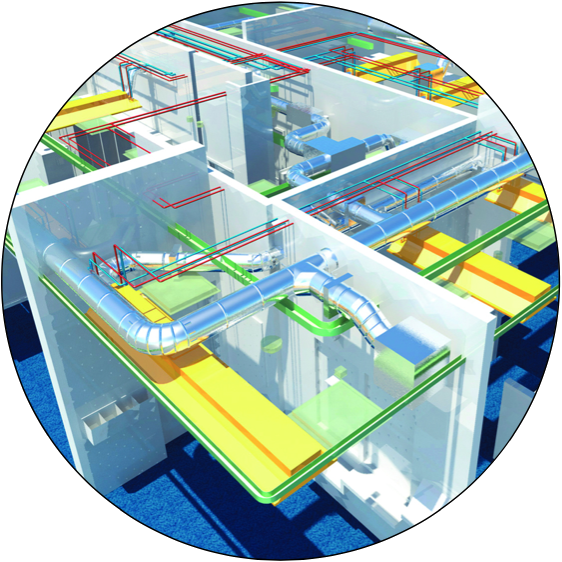
\includegraphics[width=\textwidth]{img/bim2.png}\\
		Building Information Modeling (BIM)
	\end{minipage}
	\hfill
	\begin{minipage}{.3\textwidth}
		\centering
		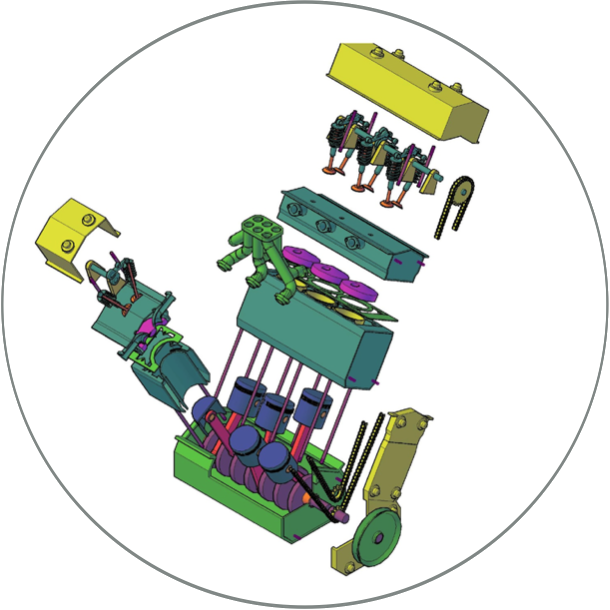
\includegraphics[width=\textwidth]{img/cad2.png}\\
		Conception Assistée par Ordinateur (CAO)
	\end{minipage}
	\hfill
	\begin{minipage}{.3\textwidth}
		\centering
		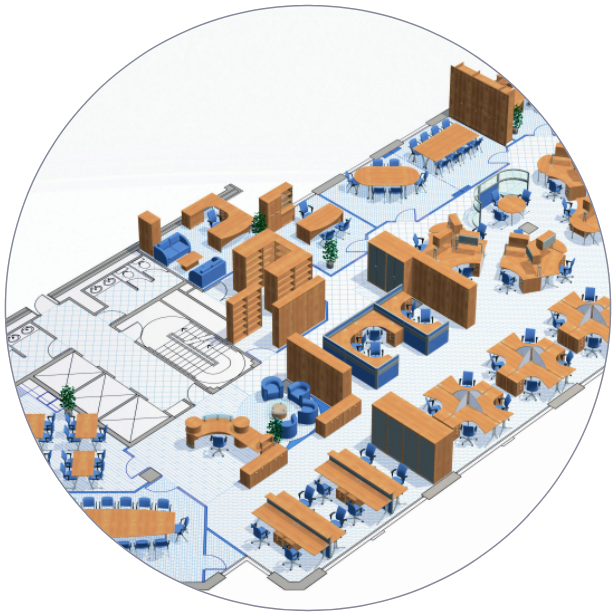
\includegraphics[width=\textwidth]{img/spaceplanning2.png}\\
		Aménagement \\ d'espace
	\end{minipage}}
	\vspace*{0.5cm}
	\centering
	
	Collaborer de manière distante sur une scène 3D
\end{frame}

%\begin{frame}{Besoins pour collaborer}
%Accompagner un groupe de 
%participants dans la réalisation d'une tâche en fournissant une 
%interface vers un environnement partagé :
%\begin{itemize}
%	\item coordination 
%	%: harmonisation des tâches, des rôles et du calendrier dans 
%	%un système simple
%	\item coopération 
%	%: résoudre des problèmes dans des environnements 
%	%complexes (impossible seul ou beaucoup plus efficace à plusieurs)
%\end{itemize}
%%Collaboration centrée activité \cite{Gotta2007} et par équipe 
%%\cite{Callahan2008}.
%
%Utilisation d'un Système d'Edition Collaborative (SEC) en temps-réel sur un 
%document (3D)
%
%Maintien de la cohérence et respect de l'intention
%%Un SEC en temps réel permet à plusieurs utilisateurs de 
%%visualiser et d'éditer de manière simultanée le même document (texte, image, 
%%objet 3D)
%
%EVC3D : réseau + systèmes distribués + 3D + interface utilisateur
%\end{frame}



\subsection{Problématique}

\begin{frame}{}
	\begin{textblock*}{95mm}(3.3cm,0.5\textheight)
		\centering \large
		\textbf{ {\color{Purple}Comment engager toutes les ressources \\ à 
		disposition 
		lors de la collaboration  sur le web?}}
	\end{textblock*}
\end{frame}



\subsection{État de l'art}


\begin{frame}
\centering

\only<1>{
	\inputTikZ{1.1}{img/tikz/namewithpics.tex}
}
\only<2>{
	\inputTikZ{1.1}{img/tikz/conception3D.tex}
}

\only<3>{
	\inputTikZ{1.1}{img/tikz/archcomm.tex}
}

\only<4>{
	\inputTikZ{1.1}{img/tikz/tracabilite.tex}
}

\only<5>{
	\inputTikZ{1.1}{img/tikz/allwithpics.tex}
}
\end{frame}


\begin{frame}{}
\renewcommand{\baselinestretch}{0.9} 
\begin{textblock*}{65mm}(8mm,0.15\textheight)
	\only<1->{
	\begin{exampleblock}{\centering Q1}
		\centering \small	
		Quelle \textbf{architecture réseau} propose une gestion efficace,  robuste et 
		temps 
réel des données 3D dans un environnement \textbf{web}?
	\end{exampleblock}}
\end{textblock*}

\begin{textblock*}{65mm}(90mm,0.15\textheight)
	\only<2->{
	\begin{exampleblock}{\centering Q2}
		\centering \small 
		Quelle architecture logicielle confère une \textbf{traçabilité} des 
	données conforme aux règles métiers liées à la manipulation d'objets 3D ?
	\end{exampleblock}}
\end{textblock*}

\begin{textblock*}{60mm}(10mm,0.65\textheight)
	\only<3->{
	\begin{exampleblock}{\centering Q3}
		\centering \small 
		Quels sont les mécanismes assurant à l'utilisateur d'être \textbf{autonome} 
		tout en 
		collaborant ?
	\end{exampleblock}}
\end{textblock*}

\begin{textblock*}{60mm}(93mm,0.65\textheight)
	\only<4->{
	\begin{exampleblock}{\centering Q4}
		\centering \small 
		Comment garantir le \textbf{respect des règles métiers} liées à la 
		manipulation 
		d'objets 3D lors de l'implantation?
	\end{exampleblock}}
\end{textblock*}

\begin{textblock*}{70mm}(48mm,0.9\textheight)
	\only<5->{
	\begin{exampleblock}{\centering Q5}
		\centering \small 
		Quelles sont les \textbf{critères} permettant d'évaluer un tel système de 
		manière quantitative ? qualitative ? 
	\end{exampleblock}}
\end{textblock*}

\begin{textblock*}{95mm}(3.3cm,0.5\textheight)
	\centering \large
	\textbf{ {\color{Purple}Comment engager toutes les ressources \\ à disposition 
			lors de la collaboration sur le web ?}}
\end{textblock*}

\end{frame}



%!TEX root = presentation.tex
\section{Approche orientée états}

\begin{frame}
	\begin{minipage}{0.5\columnwidth}
		\tableofcontents[
		currentsubsection,
		sectionstyle=show/shaded,
		subsectionstyle=show/show/hide,
		]
	\end{minipage}\hfill
	\begin{minipage}{0.5\columnwidth}
		\inputTikZ{0.7}{img/tikz/approche1.tex}
	\end{minipage}
\end{frame}

\subsection{Architecture hybride orientée états}


\begin{frame}{Quelles sont les architectures possibles dans un EVC ?}
\noindent
		\begin{minipage}{.1\columnwidth}
			\inputTikZ{.7}{img/tikz/legende.tex}
		\end{minipage}
\begin{minipage}{.45\columnwidth}
			\small
			
			\hspace*{1cm}\inputTikZ{0.8}{img/tikz/centralise.tex}
			
			\begin{itemize}
				\item Gestion concurrence/cohérence facilitée
				\item Possible goulot d'étranglement
			\end{itemize}
	\end{minipage}
\begin{minipage}{0.43\columnwidth}
		\only<2>{	\small
			\hspace*{1cm} \inputTikZ{0.8}{img/tikz/decentralise.tex}
			
			\begin{itemize}
				\item Transmission des données directes
				\item Données distribuées
			\end{itemize}}
	\end{minipage}

\only<1>{
	\separatingline{\columnwidth}
\begin{block}{Collaborer plus directement}
	Pourquoi passer par un intermédiaire (serveur) ?
\end{block}
}
\only<2>{
	\separatingline{\columnwidth}
	
\begin{block}{Faciliter la maintenance et le suivi des données}
	Que se passe-t-il s'il n'y a pas de fournisseur de données ?
\end{block}
}
\end{frame}
\begin{frame}{Quelles sont les architectures possibles dans un EVC ?}
\addtocounter{framenumber}{-1}
\begin{minipage}{.5\columnwidth}
	Hybride : Client-serveur + pair-à-pair
	\begin{itemize}
		\item Allègement de la charge du serveur (recherche et récupération)
		\item Répartition des responsabilités (dissémination, stockage)
	\end{itemize}
\end{minipage}\hfill
\begin{minipage}{.5\columnwidth}
		\hspace*{1cm}\inputTikZ{0.8}{img/tikz/semi_centralise.tex}
\end{minipage}

\separatingline{\columnwidth}
	
\begin{block}{Avantages pour la conception 3D sur le web}

	Favoriser les échanges directs 
	
	Augmenter la disponibilité des données
\end{block}
\end{frame}


\begin{frame}{Architecture de communication hybride orientée états 
\cite{Desprat2015a,Desprat2015b}}
\noindent


	\begin{minipage}{.48\columnwidth}
\only<1>{\inputTikZ{1}{img/tikz/archistate.tex}}
\only<2>{\inputTikZ{1}{img/tikz/broadcast.tex}}
	\end{minipage}\hfill
	\begin{minipage}{.48\columnwidth}
	
	Manipule des différentiels d'état ($st_1-st_0$). 
	\begin{itemize}
		\item Client-serveur : Accès \alert{centralisé} aux données pour la 
		persistance 
		long-terme ;
		\item Pair-à-pair : \alert{transmission directe} des données entre les 
		clients pour 
		la 
		collaboration.
	\end{itemize}
	
\end{minipage}
\end{frame}

%\begin{frame}{Modèle de distribution orienté états}
%
%	\begin{minipage}{.4\columnwidth}
%		\begin{figure}
%			\centering
%			\inputTikZ{1}{img/tikz/broadcast.tex}
%			\caption{Emission d'un message par $E$}
%			\label{fig:topo}
%		\end{figure}
%	\end{minipage}\hfill
%	\begin{minipage}{.6\columnwidth}
%		\begin{itemize}
%			\item Typologie de réseau : totalement maillé.
%			\item Message : différentiel entre deux états.
%			\item Cohérence forte : distribution des messages directe aux pairs et au 
%serveur.
%			\item Gestion de la concurrence pessimiste : mécanisme de verrou.
%		\end{itemize}
%	\end{minipage}
%
%\end{frame}


\subsection{3DState}

\begin{frame}{Implémentation de 3DState - Prototype de l'éditeur collaboratif 3D}


	\begin{minipage}{.45\columnwidth}
		Fonctionnalités
		\begin{itemize}
			\item Transformations haut niveau (translation, rotation, homothétie)
			\item Visualisation, navigation
			\item Import de modèles 3D
		\end{itemize}
	
	
	\begin{figure}[h]
		\centering
		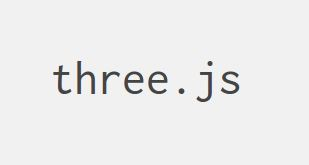
\includegraphics[height=1cm]{img/threejs.jpg}
		
\includegraphics[height=1cm]{img/webgl.png}
		
\includegraphics[height=1cm]{img/js.png}
		\label{fig:client}
	\end{figure}
	\end{minipage}\hfill
	\begin{minipage}{.55\columnwidth}
		\centering
		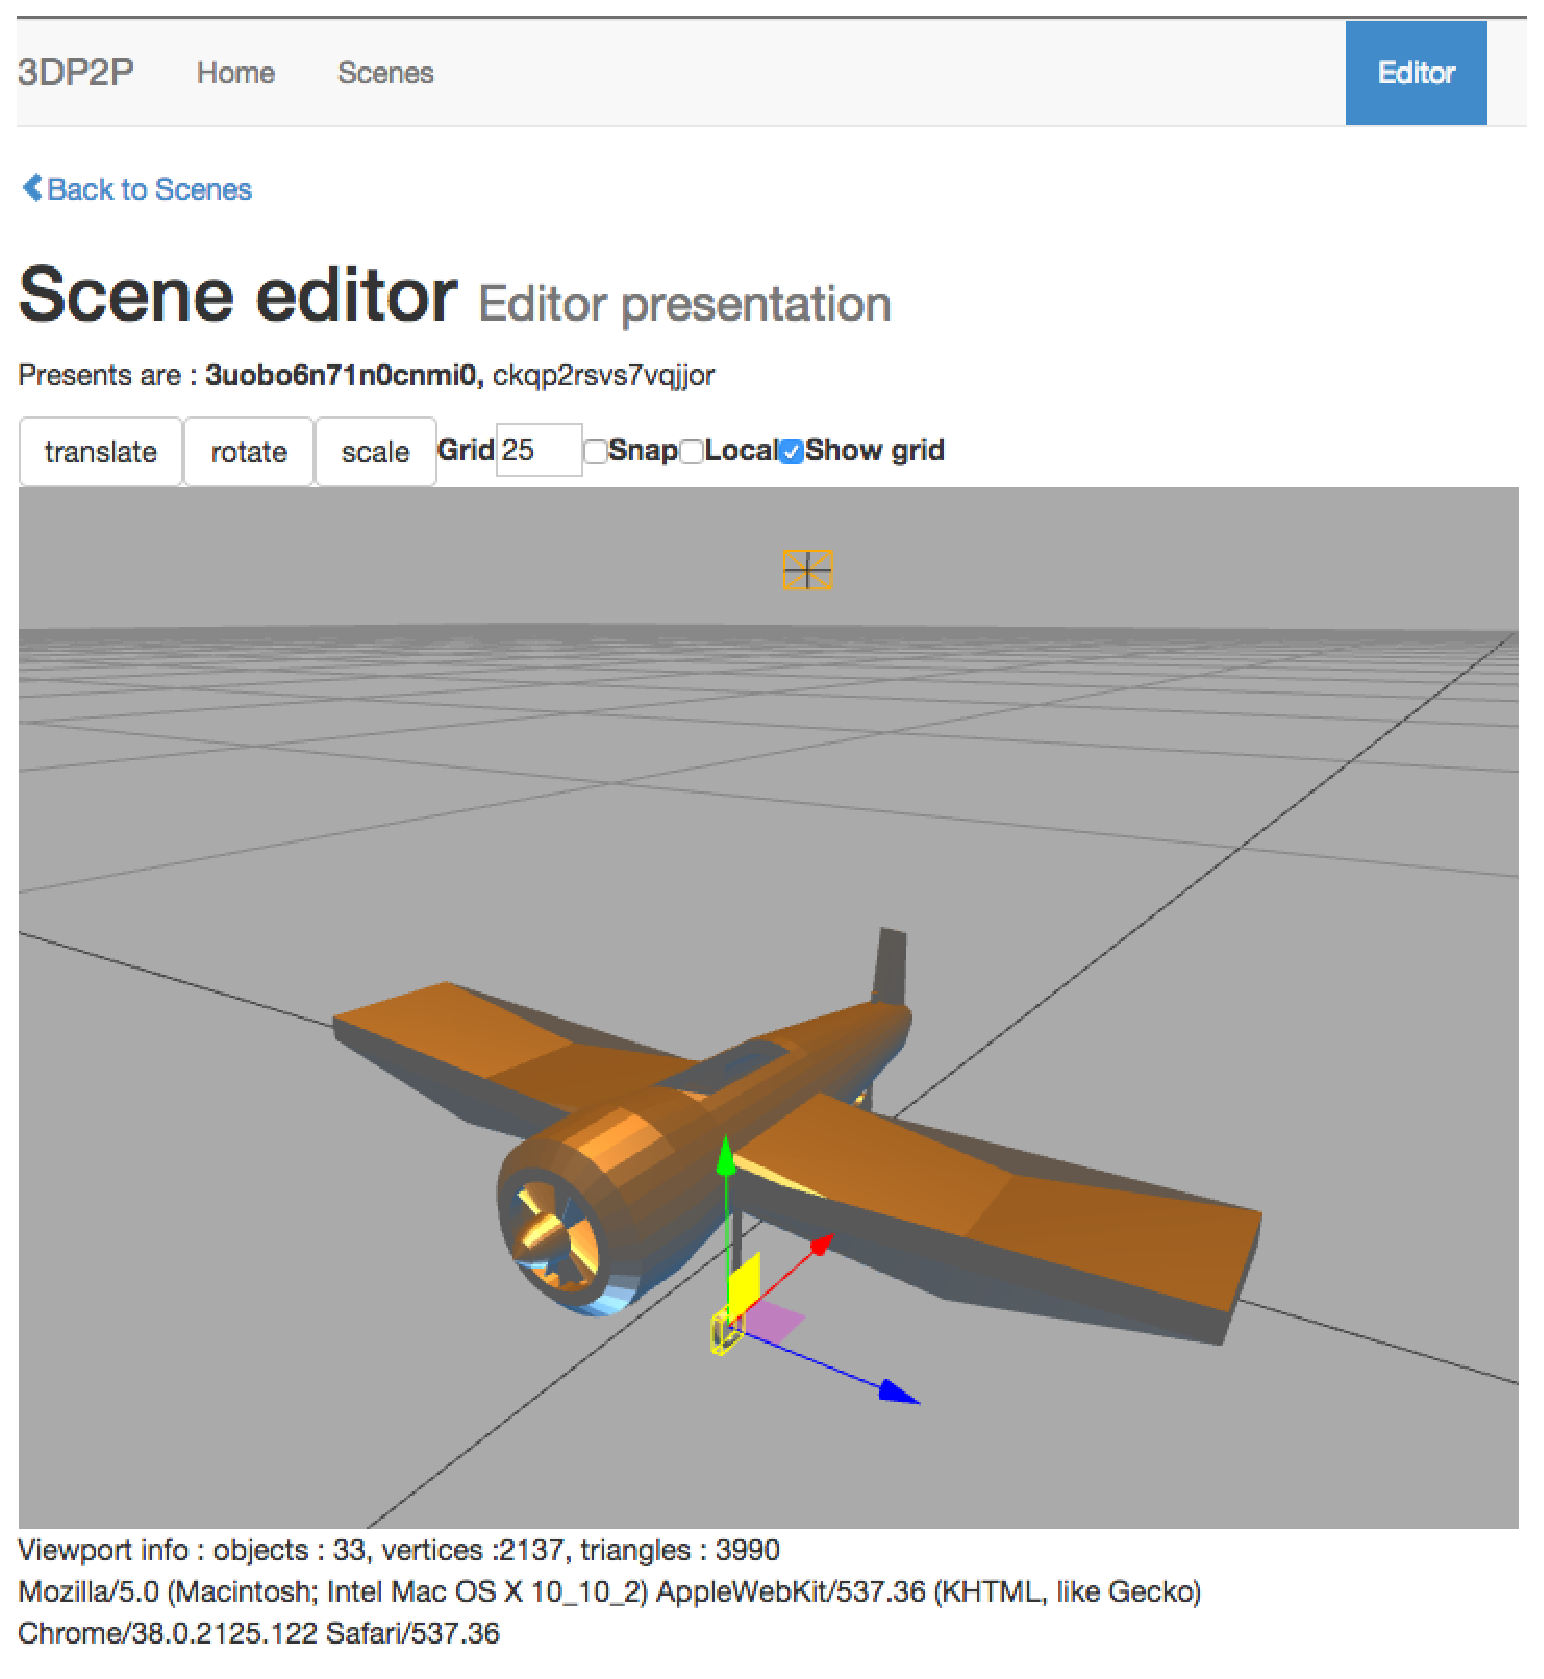
\includegraphics[width=0.8\columnwidth]{eps/editorpresentation.eps}
	\end{minipage}

\end{frame}

\subsection{Expérimentation}

\begin{frame}{Expérimentation approche orientée états}

		\begin{columns}[onlytextwidth]
			\column{0.4\textwidth}
			\begin{alertblock}{Objectif}
				Preuve de faisabilité concernant l'architecture proposée. \\
				Observations des interactions utilisateurs et réseaux\\
				Qualité de la collaboration
			\end{alertblock}
			\column{0.5\textwidth}
			
			\begin{block}{Description}
				Assemblage collaboratif des parties d'un objets.\\
				Type de réseau : réseau local\\
				Prototype : 3DState
			\end{block}
		\end{columns}
		\begin{columns}[onlytextwidth]
			\column{0.4\textwidth}
			\begin{block}{Évaluation}
				Qualité de la collaboration : cohérence, fiabilité, réactivité \\
				Résilience et robustesse du système (situations critiques)
			\end{block}
		
			\column{0.55\textwidth}
			\small
			\begin{table}[!h]
				\caption{Configuration}
				\centering
				\begin{tabular}{lccc}
					\textbf{Essai} & \textbf{Objet} & \textbf{Taille}	& 
					\textbf{NbCollab.}\\ \hline
					Wind turbine			& 6					& 1.0 MB        	& 2 \\ 
					Pick up					& 8					& 1.3 MB         	& 4	\\
					Castle from \textit{server}	& 35				& 1.3 MB        	& 4	\\
					Castle from \textit{peer}& 35 & 1.3 MB & 4 \\ \hline
				\end{tabular}
			\end{table}
		\end{columns}
\end{frame}

\begin{frame}{Résultats}
A partir des données des questionnaires et des observations:
\begin{description}
	\item[Interface utilisateur] minimale, manque de retours visuels.
	\item[Manipulation des objets] bonne évaluation sauf lors d'import de fichiers 3D 
	lourds.
	\item[Attrition] n'altère pas la qualité de la collaboration.
	\item[Globalement] Utilisateurs satisfaits (collaboration et des résultats visuels)
	\item[Qualité de la collaboration] est considérée comme \alert{temps-réel} plus 
	qu'interactive.
\end{description}

En cas de déconnexion soudaine : le système offre une bonne résilience.


%	\begin{itemize}
%		\item Croissance exponentielle des connexions
%		\item Pas de granularité 
%		\item Mise à jour du rendu à la réception d'un message.
%		\item Différentiel d'état ne permet pas de connaître l'historique des 
%		manipulations (\textit{active record}).
%	\end{itemize}
%\begin{figure}
%	\centering
%	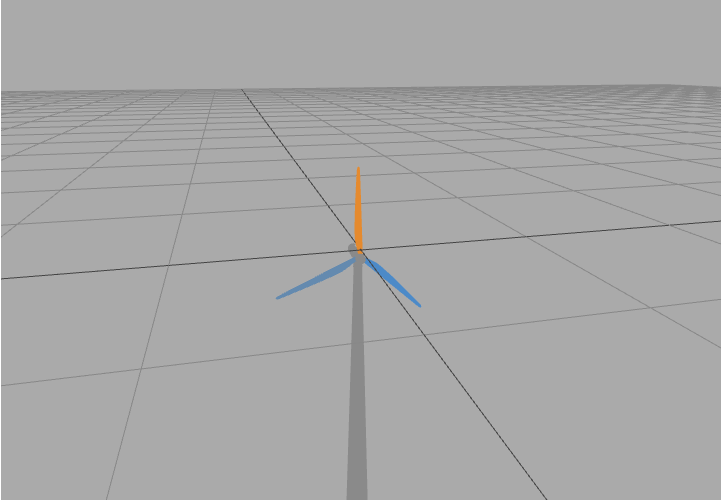
\includegraphics[width=0.3\textwidth]{eps/windturbine.png}
%	\hfill
%	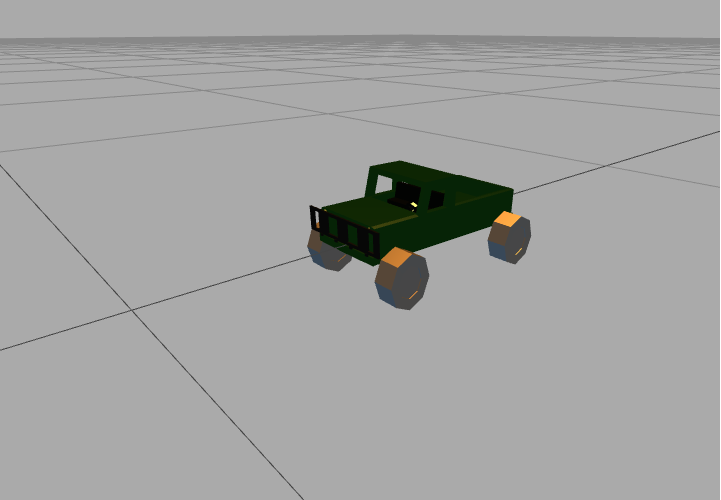
\includegraphics[width=0.3\textwidth]{eps/pickup.png}\hfill
%	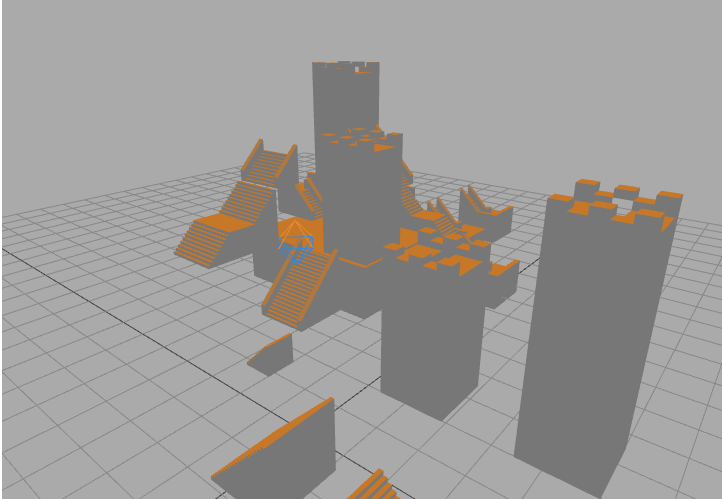
\includegraphics[width=0.3\textwidth]{eps/castle.png}\hfill
%	\caption{\label{screenshots}3D editor's captures during experiments}
%\end{figure}
\end{frame}

\begin{frame}{Bilan de l'approche orientée états}
\begin{table}[]
	\centering
	\begin{tabular}{lcc}
		\hline
		\textbf{QR}              &  \multicolumn{2}{c}{\textbf{Approche orientée états}}  
		\\ \hline
		\textbf{QR1 Réseau}      & \tickpartial   & Topologie complète, 
		diff. état       \\
		\textbf{QR2 Traçabilité} &         \fail                         & 
		Aucune                                    \\
		\textbf{QR3 Autonomie} &  \tickpartial & Stockage local 
		(session)                                 \\
		\textbf{QR4 Validité}    &         \fail                            &  
		Aucune                                     \\
		\textbf{QR5 Métriques}   & \tickpartial (quali.) \fail  (quant.)                         
		&  \multicolumn{1}{c}{\begin{tabular}[c]{@{}c@{}}Cohérence, fiabilité, 
		réactivité.\\ Robutesse et,résilience\end{tabular}}       \\ 
		\hline
	\end{tabular}
\end{table}
	\begin{description}
	\item[QR 1] L'architecture hybride permet d'augmenter la proximité entre les 
	utilisateurs. L'utilisateur est responsable de la transmission des modifications
	
	\item[QR 3] L'utilisateur stocke les informations dont il a besoin sur son client.
	
	\item[QR 5] Architecture faisable. Retours utilisateur positifs même problèmes 
	lors d'imports ou passage à l'échelle
	
	\end{description}
\end{frame}


\begin{frame}{De l'état aux événements}
	Des besoins en attente :
		\begin{itemize}
		\item Transmission par différentiel d'état : léger mais perte de l'historique des 
		manipulations (\textit{active record}).
		\item Passage à l'échelle compromis (réseau totalement maillé)
		\item Apporter plus de flexibilité à la collaboration (expertise, analyse)
	\end{itemize}
	
	Changement de paradigme : 
	\begin{itemize}
		\item Description sémantique des manipulations : introduction des 
		spécificités 
		métiers de la 3D (historisation facilitée).
		\item Améliorer le passage à l'échelle en réduisant la densité du maillage.
		\item Validation des modifications pour conserver l'intégrité du système.
	
	\end{itemize}

\end{frame}


%!TEX root = presentation.tex

\section{Approche orientée événements}

\begin{frame}
	\begin{minipage}{0.5\columnwidth}
		
		\tableofcontents[
		currentsubsection,
		sectionstyle=show/shaded,
		subsectionstyle=show/show/hide,
		]
	\end{minipage}\hfill
	\begin{minipage}{0.5\columnwidth}
		\inputTikZ{0.7}{img/tikz/approche2.tex}
	\end{minipage}
\end{frame}


\subsection{Modèle événementiel}


%\begin{frame}{Domain Driven Design}
%\begin{block}{DDD - Modélisation pilotée par le domaine \cite{Evans2003}}
%	Définir un langage et une vision partagée 
%	par tous les acteurs de l'application pour construire l'application.
%\end{block}
%	Agrégat : groupe d'objets associés considérés comme un tout vis-à-vis des 
%	modifications de données (Scène, Maillage, Géométrie)
%	
%	Agrégat racine: Seul objet accessible de l'extérieur (Scène, User) -> assurer 
%	l'intégrité du contenu à l'intérieur de l'agrégat.
%	
%	-> Proposer un langage partagé et des 
%	événements pour la manipulation et la visualisation 3D
%\end{frame}
%
%\begin{frame}{Contribution : Description des événements 3D}
%
%\begin{table}
%	\centering
%	\small
%	\caption{Exemple d'événements de 
%		l'agrégat Maillage}
%	\label{tab:extraitevent}
%	\begin{tabular}{lll}
%		\textbf{Événement}& \textbf{Dénomination} & \textbf{Description} \\ \hline
%		%\textbf{Agrégat Maillage}  &                      &             \\ \hline
%		Maillage ajouté (*)&     meshAdded                 
%		&  \begin{tabular}[c]{@{}l@{}} Un maillage a été ajouté dans\\  la Scène à 
%			partir d'une géométrie\\ de la 
%			bibliothèque \end{tabular}  \\\hline
%		Maillage déposé (*) &     meshDropped               
%		&      \begin{tabular}[c]{@{}l@{}} Un maillage a été déposé dans 
%			\\l'env. 3D de la Scène à 
%			partir \\d'une géométrie de la bibliothèque \end{tabular} \\\hline
%		Maillage supprimé & meshRemoved       &        
%		\begin{tabular}[c]{@{}l@{}} 
%			Un maillage a été 
%			supprimé \\de la Scène \end{tabular}      \\\hline
%		Maillage translaté &   meshTranslated  	 &    \begin{tabular}[c]{@{}l@{}} 
%			Un 
%			maillage a 
%			subi une translation \\dans la Scène \end{tabular}          
%	\end{tabular}
%\end{table}
%\end{frame}
%
%\begin{frame}{Event Sourcing}
%\begin{block}{ES \cite{Fowler2005EventSourcing}}
%	Enregistrer 
%	chaque modification de l'état de l'application sous la forme d'un 
%	événement.
%\end{block}
%Événement : s'applique à un agrégat, possède un type et des paramètres.
%
%Exemple: $AggScene1::meshAdded(''cube1'',geometry1)$
%
%-> Journal d'événements = source unique de vérité dans 
%l'application
%\end{frame}
%
%\begin{frame}{Command Query Responsability Segregation}
%\begin{block}{CQRS \cite{Young2009}}
%	Séparer : 
%	\begin{itemize}
%		\item la partie commande (écriture) : validation des règles métiers
%		\item de la partie requête (lecture) dans une application : passage à 
%		l'échelle, cohérence éventuelle.
%	\end{itemize}
%\end{block}
%
%La collaboration implique une forte demande partie écriture (SEC) et partie
%lecture (visualisation collaborative à synchronicité variable)
%
%
%-> Valider toute donnée entrante (utilisateur ou réseau) selon les 
%règles métiers définies. 
%
%-> Flexibilité de la visualisation du contenu généré
%avec les projections.
%\end{frame}
\begin{frame}{Patron de conception adaptés}
\only<1->{
	\begin{textblock*}{65mm}(0.05\textwidth,0.2\textheight)
		\begin{exampleblock}{DDD \cite{Vernon2013}}
			\begin{itemize}
				\item Langage partagé
				\item Contexte
				\item Règles métier
			\end{itemize}
		\end{exampleblock}
	\end{textblock*}
	
	\begin{textblock*}{65mm}(0.4\textwidth,0.2\textheight)
		\begin{exampleblock}{ES \cite{Fowler2003}}
			\begin{itemize}
				\item Un changement = un événement
				\item Événements immuables
				\item Support de l'historique
			\end{itemize}
		\end{exampleblock}
	\end{textblock*}
	
	\begin{textblock*}{65mm}(0.8\textwidth,0.2\textheight)
		
		\begin{exampleblock}{CQRS \cite{Young2010}}
			\begin{itemize}
				\item Séparer écriture / lecture
				\item Validation des données 
				\item Cohérence éventuelle 
			\end{itemize}
		\end{exampleblock}
		
	\end{textblock*}
}
\only<2>{
	\begin{textblock*}{15cm}(0.05\textwidth,0.55\textheight)
		
		\begin{exampleblock}{Définition des événements}
			
			Création du langage partagé à partir des observations des précédentes 
			expérimentations.\\
			Définition du contexte pour tous les objets liés à l'application.\\
			Définitions des événements associés à ces objets.
		\end{exampleblock}
		
	\end{textblock*}
	
	\begin{textblock*}{15cm}(0.05\textwidth,0.82\textheight)
		
		\begin{exampleblock}{CQRS+ES}
			
			Favoriser l'autonomie de l'utilisateur.\\
			Proposer différentes vues des mêmes données (3D, monitoring, 
			historique)\\
			Approche faiblement couplée adaptée à la collaboration (forte demandes 
			en 
			écriture et en lecture)
		\end{exampleblock}
		
	\end{textblock*}
}
\end{frame}

\begin{frame}{Modèle général \cite{Desprat2016}}
\centering
		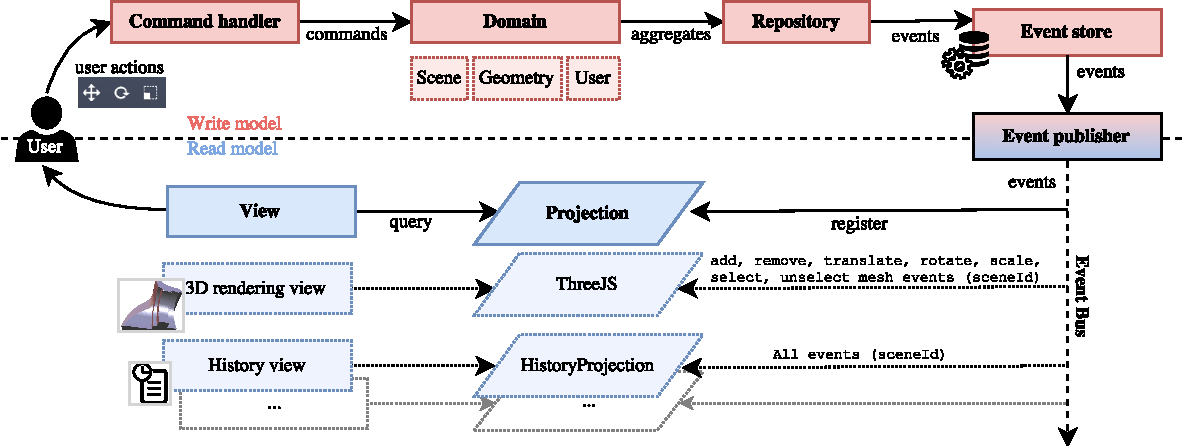
\includegraphics[width=0.9\columnwidth]{eps/cqrs3.pdf}

\end{frame}


\begin{frame}{Modèle général : exemple (translation d'un cube par User A)}

	\begin{figure}
		\centering
		\includegraphics[width=0.5\columnwidth]{eps/example10.eps}
	
	\end{figure}

\textit{Publié dans }
\end{frame}



\begin{frame}{Architecture réseau hybride orientée \cite{Desprat2017}
événements}
	{\centering
	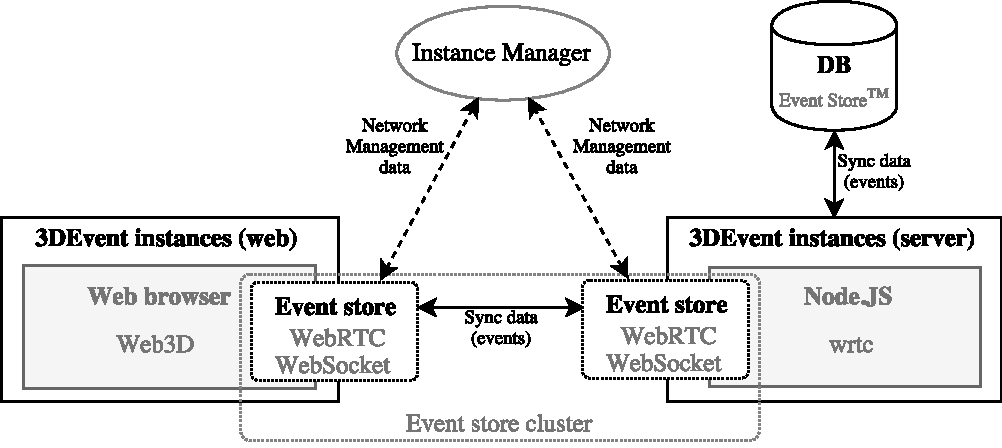
\includegraphics[width=0.7\columnwidth]{eps/archi.pdf}}


\begin{itemize}
	\item Améliorer le passage à l'échelle en intégrant le modèle événementiel
	\item Réduire les contraintes de collaboration : concurrence optimiste, réseau 
	moins dense
\end{itemize}

\end{frame}

\subsection{Prototype 3DEvent}

\begin{frame}{3DEvent - Prototype de l'éditeur collaboratif 3D}
	\begin{minipage}{.5\columnwidth}
	Fonctionnalités
	\begin{itemize}
		\item Transformations haut niveau (t,r,h)
		\item Visualisation, navigation
		\item Import de modèles 3D
	\end{itemize}
	Intégration CQRS+ES
	\begin{itemize}
		\item Interface orientée tâche 
		\item Sélection fantôme
	\end{itemize}
	\end{minipage}\hfill
	\begin{minipage}{.5\columnwidth}
		\begin{figure}
			\centering
			\includegraphics[width=\columnwidth]{eps/1translatehisto.eps}
			\caption{Translation // historique}
		\end{figure}
	\end{minipage}
\end{frame}



\begin{frame}{Expérimentation approche orientée événements}
		\begin{columns}[onlytextwidth]
		\column{0.48\textwidth}
		\begin{alertblock}{Objectif}
			Intégration du modèle événementiel possible\\
			Efficacité dans la réalisation collaborative\\
			Possibilité d'analyse des données
		\end{alertblock}
		\column{0.5\textwidth}
		
		\begin{block}{Description}
			Assemblage collaboratif de modèles 3D ou création de scène libre.\\
			Internet (hétérogène) \\
			Prototype 3DEvent.\\
		\end{block}
	\end{columns}

	\begin{columns}[onlytextwidth]
		\column{0.48\textwidth}
			\begin{block}{Critères d'évaluation}
				\begin{itemize}
					\item Qualité de la collaboration : cohérence, fiabilité, réactivité
					\item Efficience : temps et sentiment d'efficacité
				\end{itemize}
			\end{block}
		\column{0.55\textwidth}
			\scriptsize
			\begin{table}[ht]
			\centering
			\caption{Modèles}
			\begin{tabular}{cccc}
				\textbf{Modèle}  & \textbf{Nb parties} &  \textbf{Triangles} & 
				\textbf{Taille 
				tot.}  \\ \hline
				Rotor      &   10  &    62k & 4Mo \\
				Camera box        &   12  &    67k & 5Mo        \\
				Car      &   16  &      170k & 8Mo \\ 
				Living room      &   16  &      200k & 9Mo \\\hline
			\end{tabular}
		\end{table}
	\end{columns}
\end{frame}

\subsection{Résultats et discussion}
\begin{frame}{Résultats des questionnaires}

	\centering
	\includegraphics[width=\columnwidth]{eps/questionnaire.eps}


\end{frame}

\begin{frame}{Analyse des données}

	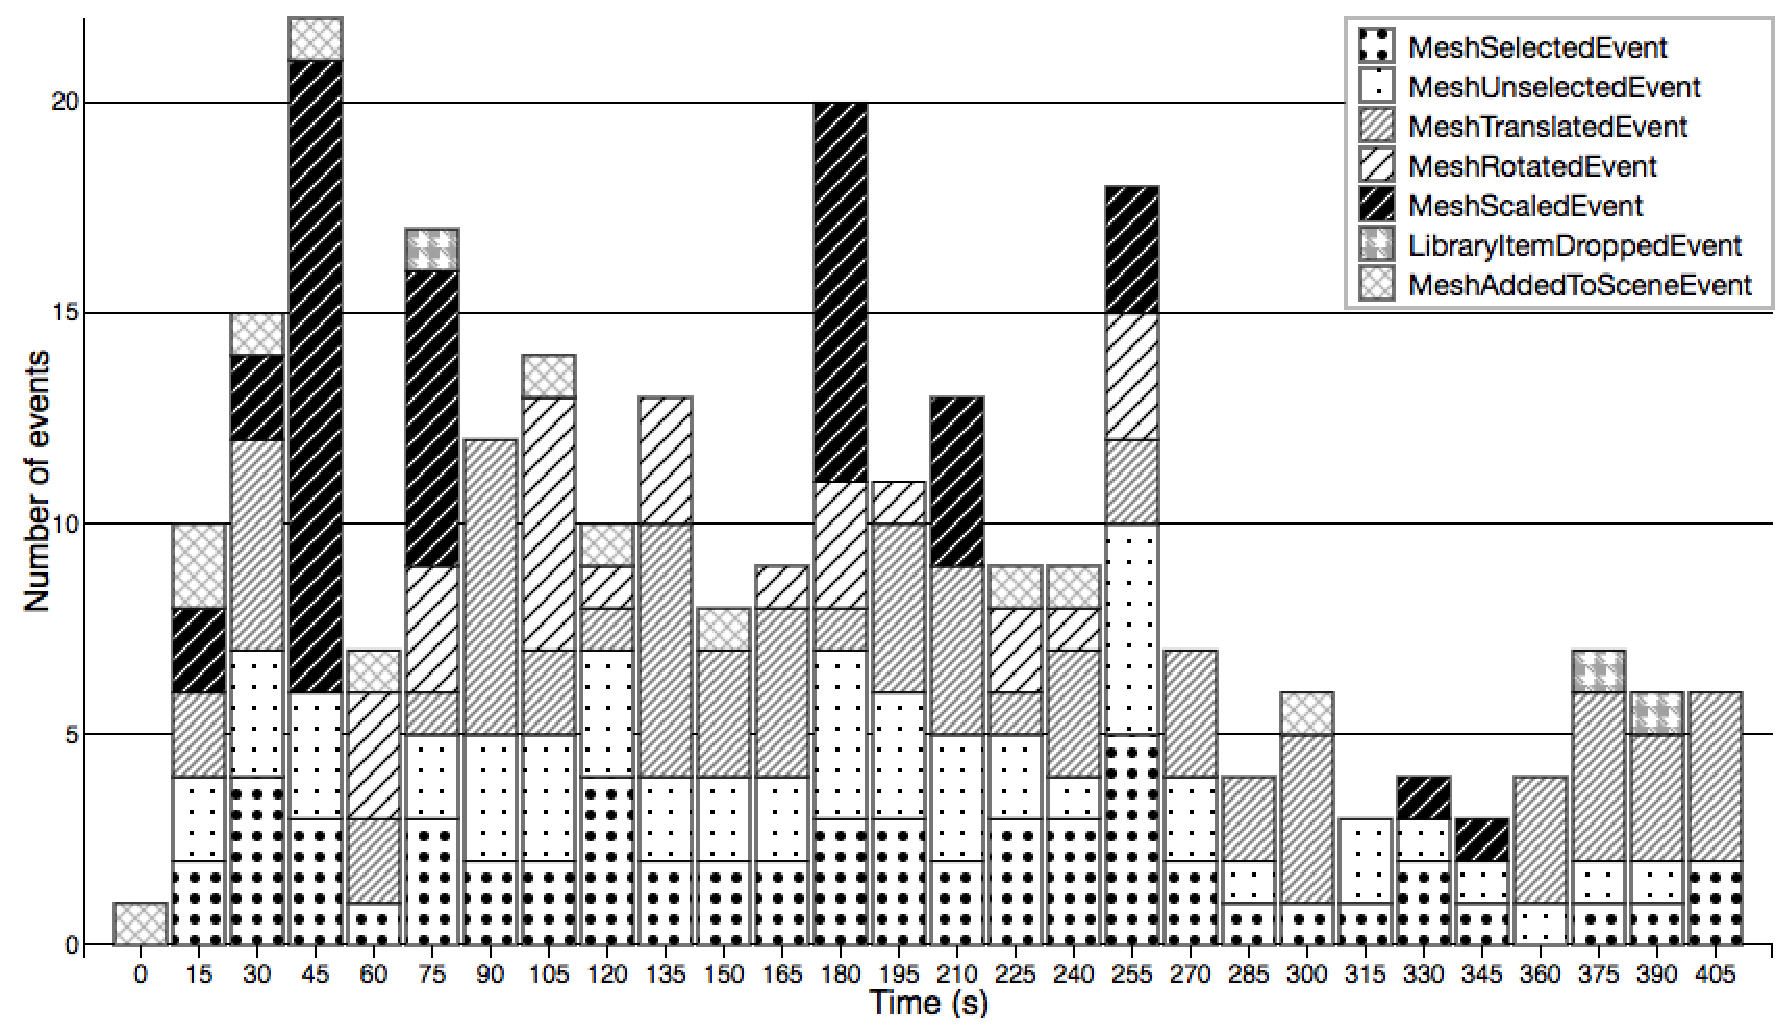
\includegraphics[width=0.8\textheight]{eps/byevents.eps}\\
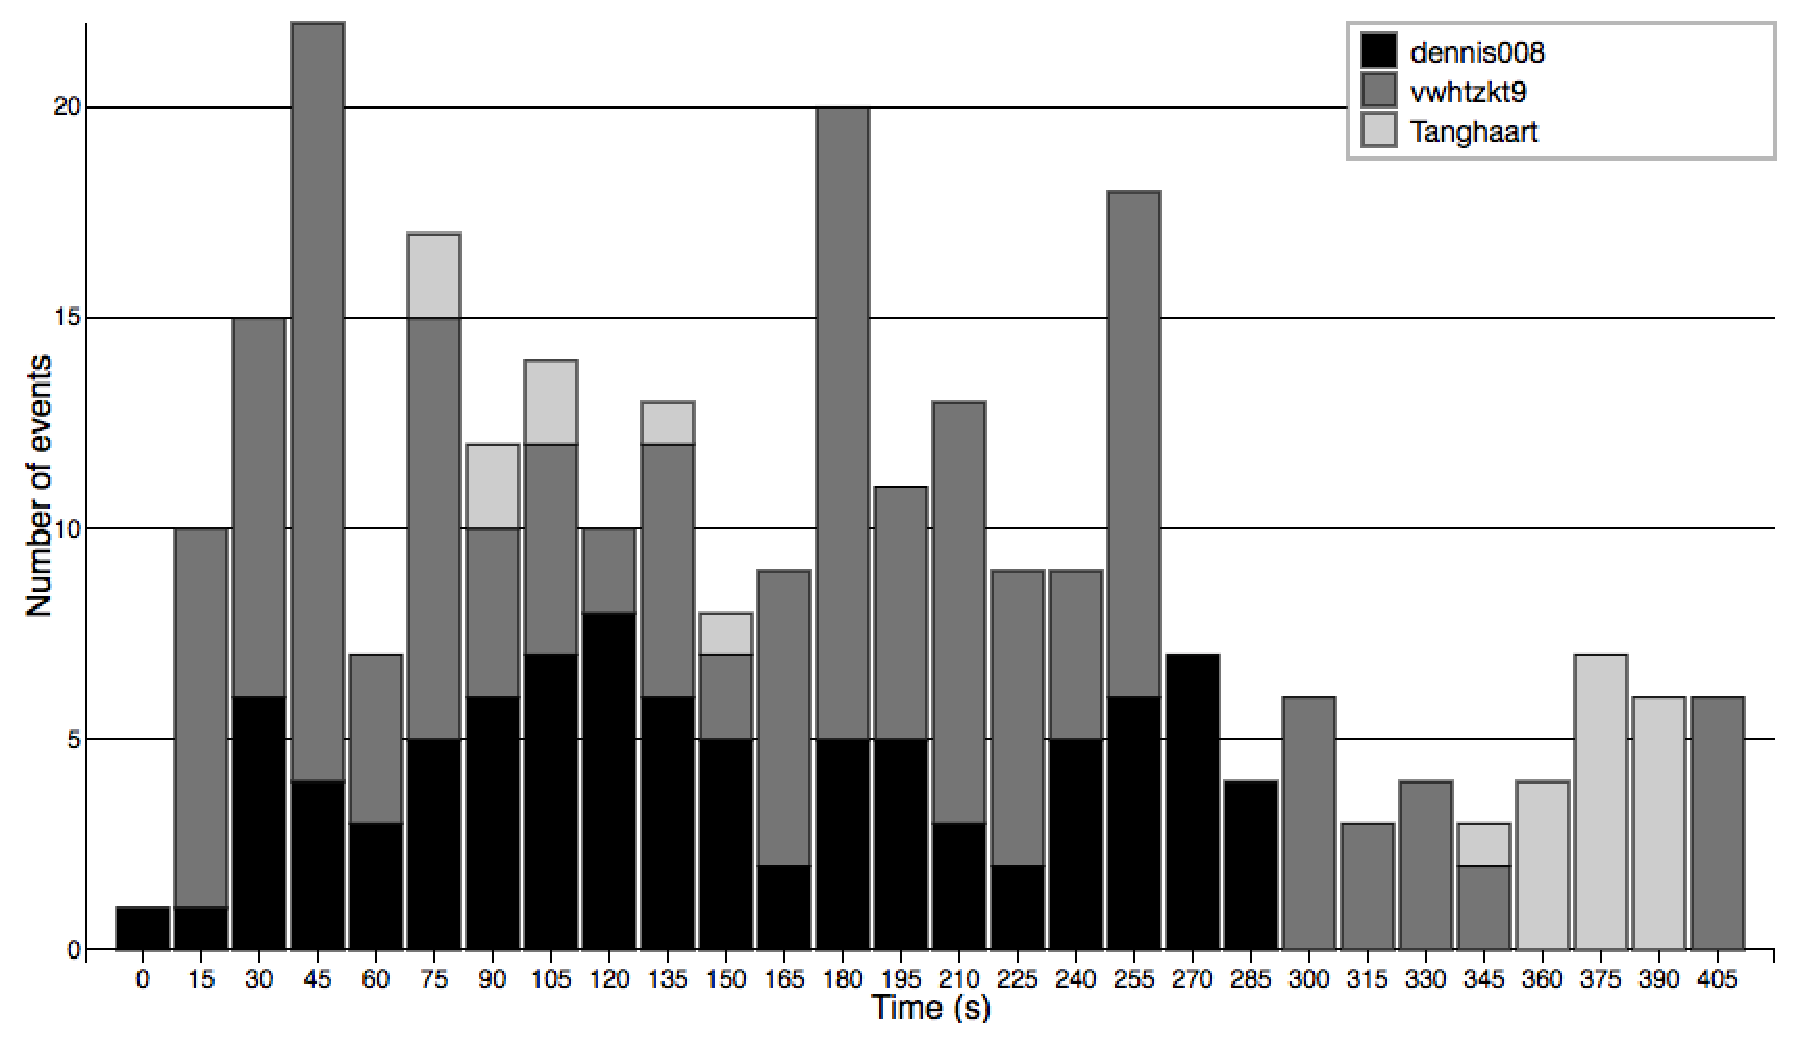
\includegraphics[width=0.8\textheight]{eps/byuser.eps}

\end{frame}

\begin{frame}{Bilan de l'approche orientée événements}
\begin{table}
	\begin{tabular}{lcc}
	\hline
	\textbf{QR}              & \multicolumn{2}{c}{\textbf{Approche orientée 
	événements}}  \\ 
	\hline
	\textbf{QR1 Réseau}      & \tick                             & Maillage partiel, flexibilité 
	(instances serveur)      \\
	\textbf{QR2 Traçabilité}  &          \tick                        & DDD et Event 
	Sourcing             \\
	\textbf{QR3 Autonomie}   & \tick                       & Stockage local 
	(haute dispo : donnnées, métier)      \\
	\textbf{QR4 Validité}    &     \tick                           &   DDD et CQRS               
	\\
	\textbf{QR5 Métriques}   & \tick (quali.)   \tickpartial 
	(quant.)                        &  Cohérence, Fiabilité, Robustesse, 
	Utilisabilité                           
	\\ 
	\hline
\end{tabular}
\end{table}
	\begin{description}

	\item[QR 2] La traçabilité est fournie par l'ES associée à la méthode DDD : 
	langage partagé de la 3D. ES fournit des données immuables et  
	fonctionnellement viables.
	
	\item[QR 3] L'utilisateur est rendu autonome par le fait de déporter CQRS et 
	ES 
	sur le client (traditionnellement client-serveur)
	
	\item[QR 4] Règles métiers fournies en amont par le DDD, validées par la 
	partie commande de CQRS
	
	%Comment les 
	%utilisateurs recoivent la chose....
\end{description}
\end{frame}

\begin{frame}{Testabilité de l'environnement virtuel collaboratif}
\begin{description}
	
	\item[QR 5] Quelles sont les critères permettant 
	d'évaluer un tel système de manière quantitative ? Qualitative ? 
	%Comment les 
	%utilisateurs recoivent la chose....
	
\end{description}
%Design and test DVEs
%\cite{Valadares2016}

%An architecture for client virtualization: A case study
Virtualisation complexe : WebRTC est une technologie récente \cite{Haque2016}


Nécessite l'intégration du modèle événementiel dans un logiciel de simulation.

De nombreuses variables : nombre de n\oe uds, types de scénarios, bande 
passante, taille des modèles 3D.

\begin{description}
	\item[temps de dissémination] d'un événement à travers le réseau
	\item[réactivité] face à la charge (nombre d'événements traités / seconde)
\end{description}



\end{frame}



%!TEX root = presentation.tex
\section{Conclusion}
\subsection{Rappel des contributions}
\begin{frame}{Résumé}

	\begin{textblock*}{95mm}(3.5cm,0.2\textheight)
	\centering \large
	\textbf{ {\color{Purple}Comment engager toutes les ressources \\ à 
			disposition 
			lors de la collaboration  sur le web?}}
\end{textblock*}

\vspace*{0.5cm}
\begin{minipage}{0.5\textwidth}
	\begin{itemize}		
		\item Architecture hybride : chaque pair participe à la distribution et au 
		stockage en temps réel et de manière égalitaire.
		\item Modèle événementiel : taxonomie et traçabilité des manipulations. 
		L'expertise des utilisateurs est sauvée et réutilisable.

	\end{itemize}
\end{minipage}\hfill
\begin{minipage}{0.5\textwidth}
	\vspace*{0.5cm}
	\centering
\inputTikZ{0.7}{img/tikz/approche12.tex}
\end{minipage}
\end{frame}


\begin{frame}{Questions de recherche}
\begin{table}
	\begin{tabular}{lcc}
		\hline
		\textbf{QR}              & \textbf{Approche orientée états} & \textbf{Approche 
			orientée événements} \\ \hline
		\textbf{QR1 Réseau}      &\tickpartial                         &  
		\tick                         \\
		\textbf{QR2 Traçabilité} &     \fail                & \tick                                  \\
		\textbf{QR3 Autonomie}   & \tickpartial                           & \tick                 \\
		\textbf{QR4 Validité}    &         \fail                         &\tick                      \\
		\textbf{QR5 Métriques}  &  \tickpartial (quali.) \fail  (quant.) & \tick (quali.)  
		\tickpartial  (quant.)       \\ \hline
	\end{tabular}
\end{table}

\end{frame}

\subsection{Perspectives}
\begin{frame}{Usages potentiels}
	La conception d'un modèle événementiel à travers l'implémentation d'une 
	plateforme 
	comme 3DEvent peut servir d'autres applications 
	asynchrones, distribuées et orientées événements.
	\begin{itemize}
		\item Application au \textbf{versionnage 3D collaboratif }avancé.
		\item \textbf{Création de scénarios} artificiels ou sur la base de traces 
		utilisateurs 
		intégrant le métier (jeux sérieux).
		\item \textbf{Traçage utilisateur et \textit{crowdsouring}} pour repérer des 
		zones d'intérêt ou proposer des résumés d'activité.
		\item Concevoir des \textbf{audits et  des outils de surveillance} pour les 
		données 
		3D issues de la collaboration.
		
	\end{itemize}
\end{frame}




\begin{frame}{Perspectives}
	Comparaison quantitative des deux approches (mêmes 
	interface/scénario/réseau)
	
	Virtualisation des comportements collaboratifs \cite{Haque2016}\cite{Erb2014}
	
	Gestion des conflits (super n\oe uds)
	\cite{Klamer2013a} % Conflict resolution event sourcing 
	\cite{Baldoni2007}
	
	
	Compression 3D \cite{Maglo2013a} (avec événements) 
\end{frame}
\section{}
\begin{frame}[plain,allowframebreaks,noframenumbering]{References}
\tiny
\bibliography{mendeley}
\bibliographystyle{alpha-fr}

\end{frame}

\end{document}